%Frame 68 -> 70
%%%%%%%%%%%%%%%%%%%%%%%%%%%%%%%%%%%%%%%%%%%%%%%%%%%%%%%%%%%%%%%%%%%%%%%%%%%%%%%%%%%%%%%%%%%%%%%%%%%%%%%%%%%%%%%%%%%%%%%%
\frame{
%{\color{isered}If we augment $ p $ we hold the level but we lose power!}\\
\color{isegreen}
\textbf{Example}\\
$ \varepsilon_t\sim$ MA(1): \hspace{1.5cm} $\varepsilon_t = \beta \xi_{t-1} + \xi_t
, \qquad \xi_t$ i.i.d. $(0,\sigma^2) $
\begin{eqnarray*}
\operatorname{Var}(\varepsilon_t) &=& \sigma^2(1+\beta^2) \\
\gamma_1(\varepsilon_t) &=& \operatorname{Cov}(\varepsilon_t,\varepsilon_{t-1}) = \beta \sigma^2 \\
\gamma_{\tau}(\varepsilon_t) &=& 0 \mbox{ for } \tau \ge 2\\
\end{eqnarray*}
Hence the ACF of $ \varepsilon_t $ is:
\begin{equation}
\rho_\tau(\varepsilon_t) = \left\{ \begin{array}{ll}
                     \frac{\beta}{1+\beta^2} & \mbox{if} \:\: \tau = 1 \\
                     0        & \mbox{if} \:\: \tau \ge 2. \\
                    \end{array} \right.
\end{equation}
}

%Frame 69 -> 71
%%%%%%%%%%%%%%%%%%%%%%%%%%%%%%%%%%%%%%%%%%%%%%%%%%%%%%%%%%%%%%%%%%%%%%%%%%%%%%%%%%%%%%%%%%%%%%%%%%%%%%%%%%%%%%%%%%%%%%%%
\frame{
\bigskip
\color{isegreen}
For the process
\begin{equation}
X_t = \alpha X_{t-1} + \varepsilon_t = \alpha X_{t-1} + \beta \xi_{t-1} + \xi_t
\label{gl13.32}
\end{equation}
we make simulations for the ADF test.
\begin{table}
\begin{center}
\color{black}
\small
\begin{tabular}{cc|ccccc}\hline \hline
 & & \multicolumn{5}{c}{$\beta$} \\
$\alpha$ & $p$ & -0.99 & -0.90 & 0 & 0.90 & 0.99\\ \hline
1 & 3 & 0.992 & 0.933 & 0.043 & 0.100 & 0.112 \\ 
  & 11 & 0.219 & 0.111 & 0.040 & 0.050 & 0.072 \\  \hline
0.90 & 3 & 0.998 & 0.995 & 0.130 & 0.258 & 0.288 \\ 
  & 11 & 0.322 & 0.222 & 0.056 & 0.081 & 0.103 \\  \hline \hline
\end{tabular}
\caption{ADF-test: simulated rejection probability for the
process (\protect\ref{gl13.32}) with a  nominal level of 5\%
(Friedmann, 1992). \label{adfsimu}}
\end{center}
\href{https://github.com/QuantLet/SFM2-SS16-ToDo/tree/master/SFESimADF}{\quantnet{SFESimADF}}
\end{table}
}

\frame{
\begin{figure}
\begin{center}
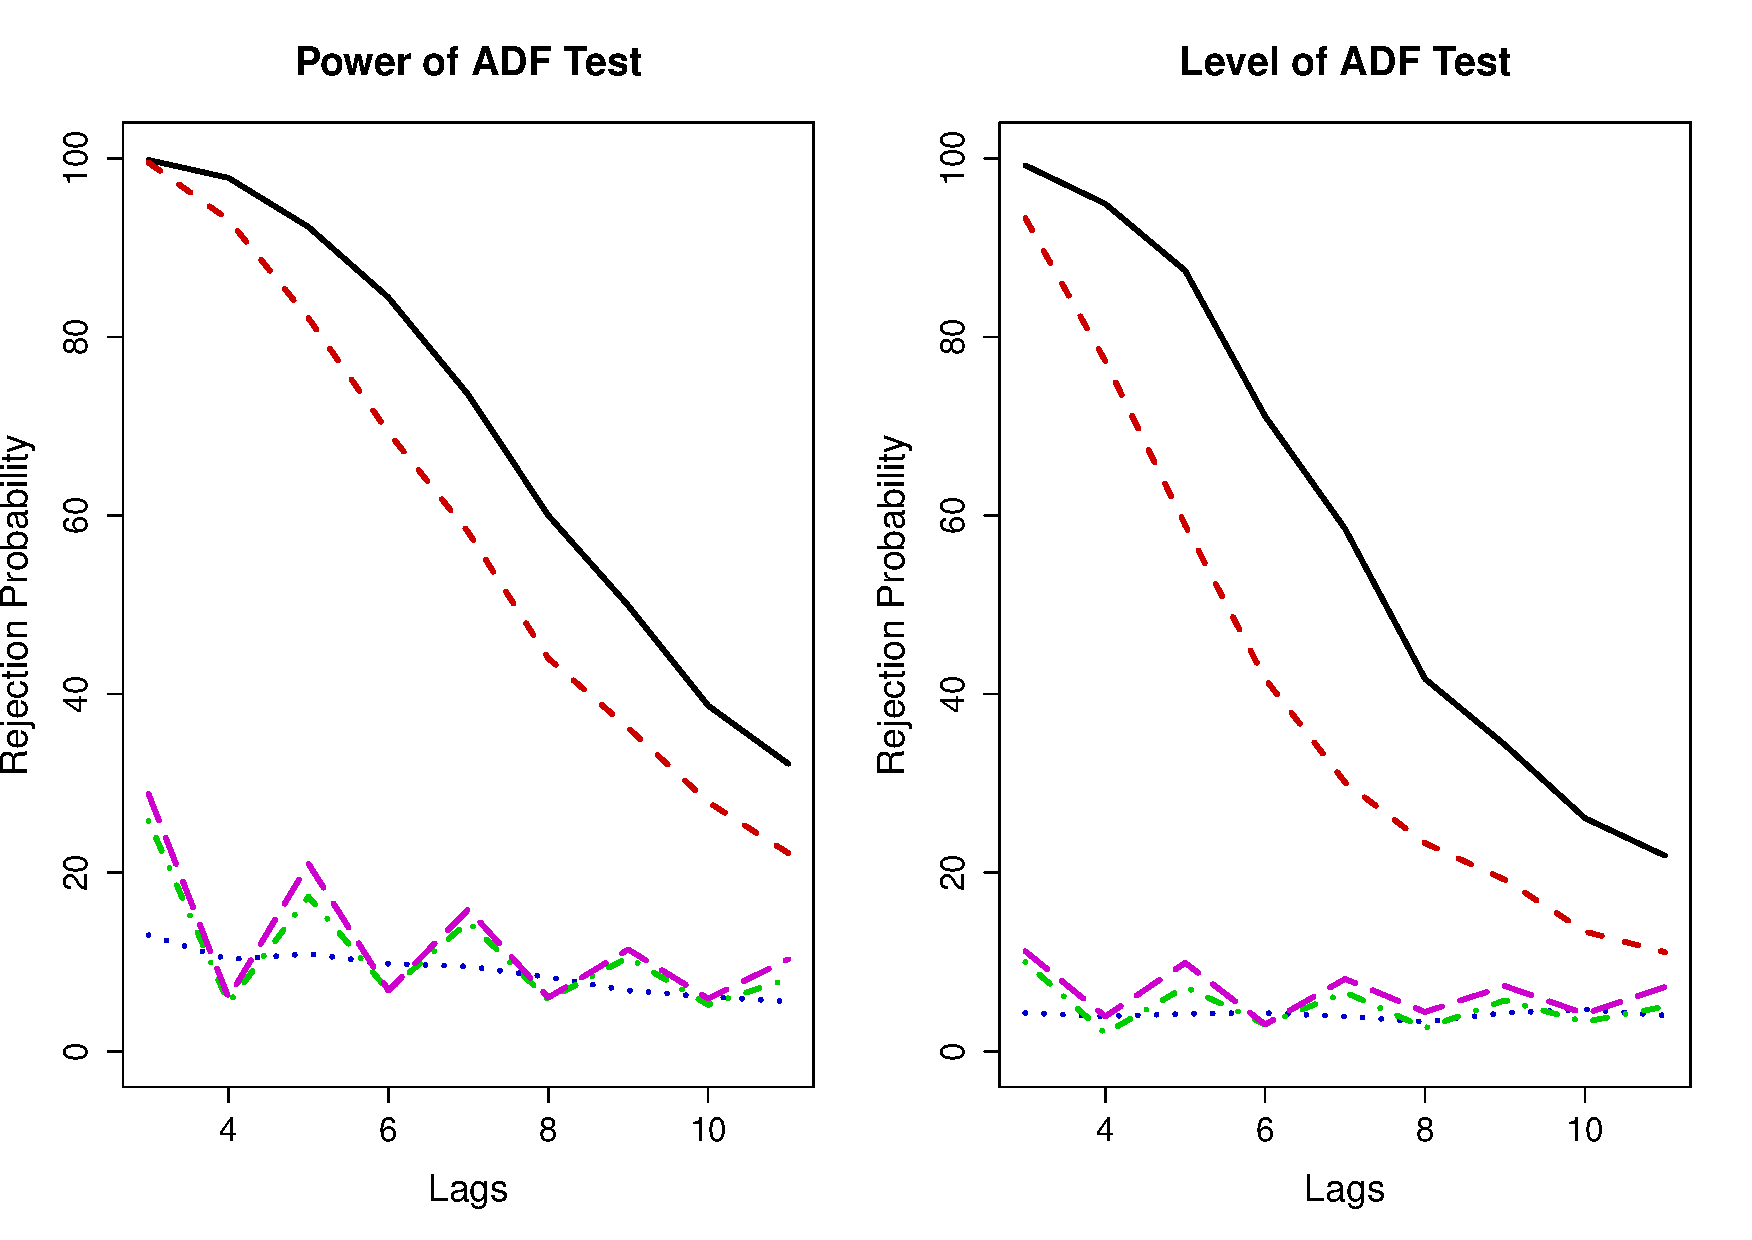
\includegraphics[scale=0.2]{figures/SFESimADF.pdf}
\caption{A plot for the level ($\alpha = 0.9$) and the power ($\alpha = 1$) of Augmented Dickey-Fuller tests.
The rejection probability for $\beta = -0.99$ (black), $\beta = -0.90$ (red), $\beta = 0$ (blue), $\beta = -0.90$ 
(green) and $\beta = -0.99$ (magenta) depends on the number of included lags ($p$).
\end{center}
\href{https://github.com/QuantLet/SFM2-SS16-ToDo/tree/master/SFESimADF}{\quantnet{SFESimADF}}
\end{figure}

Project: Update Table 44 by using R.
}